\item \points{35} {\bf Semi-supervised EM}

\def\zsi{z^{(i)}}
\def\xsi{x^{(i)}}

Expectation Maximization (EM) is a classical algorithm for unsupervised learning (\emph{i.e.,} learning with hidden or latent variables). In this problem we will explore one of the ways in which EM algorithm can be adapted to the semi-supervised setting, where we have some labeled examples along with unlabeled examples.

In the standard unsupervised setting, we have $\nexp \in \mathbb{N}$ unlabeled examples $\{x^{(1)},\ldots,x^{(\nexp)}\}$. We wish to learn the parameters of $p(x,z;\theta)$ from the data, but $\zsi$'s are not observed. The classical EM algorithm is designed for this very purpose, where we maximize the intractable $p(x;\theta)$ indirectly by iteratively performing the E-step and M-step, each time maximizing a tractable lower bound of $p(x;\theta)$. Our objective can be concretely written as:

\begin{align*}
    \ell_{\text{unsup}}(\theta) &= \sum_{i=1}^\nexp \log p(\xsi;\theta) \\
    &= \sum_{i=1}^\nexp \log \sum_{\zsi} p(\xsi,\zsi;\theta)
\end{align*}


Now, we will attempt to construct an extension of EM to the semi-supervised setting. Let us suppose we have an \emph{additional} $\tilde{\nexp} \in \mathbb{N}$ labeled examples $\{(\tilde{x}^{(1)},\tilde{z}^{(1)}),\ldots,(\tilde{x}^{(\tilde{\nexp})},\tilde{z}^{(\tilde{\nexp})})\}$ where both $x$ and $z$ are observed. We want to simultaneously maximize the marginal likelihood of the parameters using the unlabeled examples, and full likelihood of the parameters using the labeled examples, by optimizing their weighted sum (with some hyperparameter $\alpha$). More concretely, our semi-supervised objective $\ell_\text{semi-sup}(\theta)$ can be written as:
%
\begin{align*}
    \ell_\text{sup}(\theta) &= \sum_{i=1}^{\tilde{\nexp}} \log p(\tilde{x}^{(i)},\tilde{z}^{(i)};\theta) \\
    \ell_{\text{semi-sup}}(\theta) &= \ell_\text{unsup}(\theta) + \alpha \ell_\text{sup}(\theta)
\end{align*}
%
We can derive the EM steps for the semi-supervised setting using the same approach and steps as before. You are \emph{strongly encouraged} to show to yourself (no need to include in the write-up) that we end up with:

\subsubsection*{E-step (semi-supervised)}

For each $i \in \{1,\ldots,\nexp\}$, set
\begin{align*}
    Q_i^{(t)}(\zsi) := p(\zsi|\xsi;\theta^{(t)})
\end{align*}

\subsubsection*{M-step (semi-supervised)}

\begin{align*}
    \theta^{(t+1)} &:= \arg\max_\theta\left[ \sum_{i=1}^\nexp\left( \sum_{\zsi} Q^{(t)}_i(\zsi) \log \frac{ p(\xsi, \zsi;\theta) }{ Q^{(t)}_i(\zsi)}\right)  + \alpha \left(\sum_{i=1}^{\tilde{\nexp}} \log p(\tilde{x}^{(i)},\tilde{z}^{(i)};\theta)\right)\right]
\end{align*}

\begin{enumerate}
  \item\subquestionpoints{5}
\textbf{Convergence.}
First we will show that this algorithm eventually converges. In order to prove this, it is sufficient to show that our semi-supervised objective $\ell_\text{semi-sup}(\theta)$ monotonically increases with each iteration of E and M step. Specifically, let $\theta^{(t)}$ be the parameters obtained at the end of $t$ EM-steps. Show that $\ell_\text{semi-sup}(\theta^{(t+1)}) \ge \ell_\text{semi-sup}(\theta^{(t)})$.



\ifnum\solutions=1 {
  \begin{answer}
\end{answer}

} \fi

\end{enumerate}


\subsubsection*{Semi-supervised GMM}
Now we will revisit the Gaussian Mixture Model (GMM), to apply our semi-supervised EM algorithm. Let us consider a scenario where data is generated from $k \in \mathbb{N}$ Gaussian distributions, with unknown means $\mu_j \in \R^\di$ and covariances $\Sigma_j \in \mathbb{S}_+^\di$ where $j \in \{1,\ldots,k\}$. We have $\nexp$ data points $\xsi \in \R^\di, i \in \{1,\ldots,\nexp\}$, and each data point has a corresponding latent (hidden/unknown) variable $\zsi \in \{1,\ldots,k\}$ indicating which distribution $\xsi$ belongs to. Specifically, $\zsi \sim \text{Multinomial}(\phi)$, such that $\sum_{j=1}^k\phi_j = 1$ and $\phi_j \ge 0$ for all $j$, and $\xsi|\zsi \sim \mathcal{N}\left(\mu_{\zsi}, \Sigma_{\zsi}\right)$ i.i.d. So, $\mu$, $\Sigma$, and $\phi$ are the model parameters.

We also have additional $\tilde{\nexp}$ data points $\tilde{x}^{(i)} \in \R^\di, i \in \{1,\ldots,\tilde{\nexp}\}$, and an associated \emph{observed} variable $\tilde{z}^{(i)} \in \{1,\ldots,k\}$ indicating the distribution $\tilde{x}^{(i)}$ belongs to. Note that $\tilde{z}^{(i)}$ are known constants (in contrast to $\zsi$ which are unknown \emph{random} variables). As before, we assume $\tilde{x}^{(i)}|\tilde{z}^{(i)} \sim \mathcal{N}\left(\mu_{\tilde{z}^{(i)}}, \Sigma_{\tilde{z}^{(i)}}\right)$ i.i.d.


In summary we have $\nexp$ + $\tilde{\nexp}$ examples, of which $\nexp$ are unlabeled data points $x$'s with unobserved $z$'s, and $\tilde{\nexp}$ are labeled data points $\tilde{x}^{(i)}$ with corresponding observed labels $\tilde{z}^{(i)}$. The traditional EM algorithm is designed to take only the $\nexp$ unlabeled examples as input, and learn the model parameters $\mu$, $\Sigma$, and $\phi$.


Our task now will be to apply the semi-supervised EM algorithm to GMMs in order to also leverage the additional $\tilde{\nexp}$ labeled examples, and come up with semi-supervised E-step and M-step update rules specific to GMMs. Whenever required, you can cite the lecture notes for derivations and steps.


\begin{enumerate}
  \setcounter{enumii}{1}
  \item\subquestionpoints{5} \textbf{Semi-supervised E-Step.}
Clearly state which are all the latent variables that need to be re-estimated in the E-step. Derive the E-step to re-estimate all the stated latent variables. Your final E-step expression must only involve $x, z, \mu, \Sigma, \phi$ and universal constants.


\ifnum\solutions=1 {
  %
\documentclass{article}

\usepackage{graphicx}

\newcommand{\di}{{d}}
\newcommand{\nexp}{{n}}
\newcommand{\nf}{{p}}
\newcommand{\vcd}{{\textbf{D}}}

\usepackage{nccmath}
\usepackage{mathtools}
\usepackage{graphicx,caption}
\usepackage{enumitem}
\usepackage{epstopdf,subcaption}
\usepackage{psfrag}
\usepackage{amsmath,amssymb,epsf}
\usepackage{verbatim}
\usepackage[hyphens]{url}
\usepackage{color}
\usepackage{bbm}
\usepackage{listings}
\usepackage{setspace}
\usepackage{float}
\usepackage{natbib}
\definecolor{Code}{rgb}{0,0,0}
\definecolor{Decorators}{rgb}{0.5,0.5,0.5}
\definecolor{Numbers}{rgb}{0.5,0,0}
\definecolor{MatchingBrackets}{rgb}{0.25,0.5,0.5}
\definecolor{Keywords}{rgb}{0,0,1}
\definecolor{self}{rgb}{0,0,0}
\definecolor{Strings}{rgb}{0,0.63,0}
\definecolor{Comments}{rgb}{0,0.63,1}
\definecolor{Backquotes}{rgb}{0,0,0}
\definecolor{Classname}{rgb}{0,0,0}
\definecolor{FunctionName}{rgb}{0,0,0}
\definecolor{Operators}{rgb}{0,0,0}
\definecolor{Background}{rgb}{0.98,0.98,0.98}
\lstdefinelanguage{Python}{
numbers=left,
numberstyle=\footnotesize,
numbersep=1em,
xleftmargin=1em,
framextopmargin=2em,
framexbottommargin=2em,
showspaces=false,
showtabs=false,
showstringspaces=false,
frame=l,
tabsize=4,
% Basic
basicstyle=\ttfamily\footnotesize\setstretch{1},
backgroundcolor=\color{Background},
% Comments
commentstyle=\color{Comments}\slshape,
% Strings
stringstyle=\color{Strings},
morecomment=[s][\color{Strings}]{"""}{"""},
morecomment=[s][\color{Strings}]{'''}{'''},
% keywords
morekeywords={import,from,class,def,for,while,if,is,in,elif,else,not,and,or
,print,break,continue,return,True,False,None,access,as,,del,except,exec
,finally,global,import,lambda,pass,print,raise,try,assert},
keywordstyle={\color{Keywords}\bfseries},
% additional keywords
morekeywords={[2]@invariant},
keywordstyle={[2]\color{Decorators}\slshape},
emph={self},
emphstyle={\color{self}\slshape},
%
}


\pagestyle{empty} \addtolength{\textwidth}{1.0in}
\addtolength{\textheight}{0.5in}
\addtolength{\oddsidemargin}{-0.5in}
\addtolength{\evensidemargin}{-0.5in}
\newcommand{\ruleskip}{\bigskip\hrule\bigskip}
\newcommand{\nodify}[1]{{\sc #1}}
\newcommand{\points}[1]{{\textbf{[#1 points]}}}
\newcommand{\subquestionpoints}[1]{{[#1 points]}}
\newenvironment{answer}{{\bf Answer:} \sf \begingroup\color{red}}{\endgroup}%

\newcommand{\bitem}{\begin{list}{$\bullet$}%
{\setlength{\itemsep}{0pt}\setlength{\topsep}{0pt}%
\setlength{\rightmargin}{0pt}}}
\newcommand{\eitem}{\end{list}}

\setlength{\parindent}{0pt} \setlength{\parskip}{0.5ex}
\setlength{\unitlength}{1cm}

\renewcommand{\Re}{{\mathbb R}}
\newcommand{\R}{\mathbb{R}}
\newcommand{\what}[1]{\widehat{#1}}

\renewcommand{\comment}[1]{}
\newcommand{\mc}[1]{\mathcal{#1}}
\newcommand{\half}{\frac{1}{2}}

\def\KL{D_{KL}}
\def\xsi{x^{(i)}}
\def\ysi{y^{(i)}}
\def\zsi{z^{(i)}}
\def\E{\mathbb{E}}
\def\calN{\mathcal{N}}
\def\calD{\mathcal{D}}

\usepackage{tikz}
\usepackage{bbding}
\usepackage{pifont}
\usepackage{wasysym}
\usepackage{amssymb}
\usepackage{booktabs}
\usepackage{verbatim}


%\begin{document}
\begin{answer}
semi supervised EM algorithm for Gaussian mixture model is straightforward. We have log likelihood $l_{\text{semisup}}(\theta) = l_{\text{unsup}}(\theta) + \alpha l_{\text{sup}}(\theta)$ which we wish to maximise, where here $\theta = \phi, \mu, \Sigma$. for the E-step we compute $Q_i(z_i) = p(z_i | x_i; \phi, \mu, \Sigma)$ for the unsupervised points $x_i \in \{x_1, ..., x_n\}$.

We parametrise the distribution $Q_i(z_i) \in \R^k$ for k choices of Gaussian distribution by writing
\begin{align*}
Q_i(z_i)_j = w^{(i)}_j
&= p(z_i = j | x_i; \phi, \mu, \Sigma)
\\
&= p(x|z) \frac{p(z)}{p(x)}
\\
&= p(x_i | z_i = j) \frac{p(z_i = j)}{p(x_i)}
\\
&= N(\mu_j, \Sigma_j) \frac{\phi_j}{\sum_{l=1}^k p(x_i | z_i = l) p(z_i = l)}
\\
&= \frac{ N(x_i; \mu_j, \Sigma_j) \phi_j}{\sum_{l=1}^k N(x_i; \mu_l, \Sigma_l) \phi_l}
\end{align*}
\end{answer}
%\end{document}
} \fi

  \item\subquestionpoints{10} \textbf{Semi-supervised M-Step.}
Clearly state which are all the parameters that need to be re-estimated in the M-step. Derive the M-step to re-estimate all the stated parameters.  Specifically,
derive closed form expressions for the parameter update rules for $\mu^{(t+1)}$, $\Sigma^{(t+1)}$ and $\phi^{(t+1)}$ based on the semi-supervised objective.


\ifnum\solutions=1 {
  
\documentclass{article}

\usepackage{graphicx}

\newcommand{\di}{{d}}
\newcommand{\nexp}{{n}}
\newcommand{\nf}{{p}}
\newcommand{\vcd}{{\textbf{D}}}

\usepackage{nccmath}
\usepackage{mathtools}
\usepackage{graphicx,caption}
\usepackage{enumitem}
\usepackage{epstopdf,subcaption}
\usepackage{psfrag}
\usepackage{amsmath,amssymb,epsf}
\usepackage{verbatim}
\usepackage[hyphens]{url}
\usepackage{color}
\usepackage{bbm}
\usepackage{listings}
\usepackage{setspace}
\usepackage{float}
\usepackage{natbib}
\definecolor{Code}{rgb}{0,0,0}
\definecolor{Decorators}{rgb}{0.5,0.5,0.5}
\definecolor{Numbers}{rgb}{0.5,0,0}
\definecolor{MatchingBrackets}{rgb}{0.25,0.5,0.5}
\definecolor{Keywords}{rgb}{0,0,1}
\definecolor{self}{rgb}{0,0,0}
\definecolor{Strings}{rgb}{0,0.63,0}
\definecolor{Comments}{rgb}{0,0.63,1}
\definecolor{Backquotes}{rgb}{0,0,0}
\definecolor{Classname}{rgb}{0,0,0}
\definecolor{FunctionName}{rgb}{0,0,0}
\definecolor{Operators}{rgb}{0,0,0}
\definecolor{Background}{rgb}{0.98,0.98,0.98}
\lstdefinelanguage{Python}{
numbers=left,
numberstyle=\footnotesize,
numbersep=1em,
xleftmargin=1em,
framextopmargin=2em,
framexbottommargin=2em,
showspaces=false,
showtabs=false,
showstringspaces=false,
frame=l,
tabsize=4,
% Basic
basicstyle=\ttfamily\footnotesize\setstretch{1},
backgroundcolor=\color{Background},
% Comments
commentstyle=\color{Comments}\slshape,
% Strings
stringstyle=\color{Strings},
morecomment=[s][\color{Strings}]{"""}{"""},
morecomment=[s][\color{Strings}]{'''}{'''},
% keywords
morekeywords={import,from,class,def,for,while,if,is,in,elif,else,not,and,or
,print,break,continue,return,True,False,None,access,as,,del,except,exec
,finally,global,import,lambda,pass,print,raise,try,assert},
keywordstyle={\color{Keywords}\bfseries},
% additional keywords
morekeywords={[2]@invariant},
keywordstyle={[2]\color{Decorators}\slshape},
emph={self},
emphstyle={\color{self}\slshape},
%
}


\pagestyle{empty} \addtolength{\textwidth}{1.0in}
\addtolength{\textheight}{0.5in}
\addtolength{\oddsidemargin}{-0.5in}
\addtolength{\evensidemargin}{-0.5in}
\newcommand{\ruleskip}{\bigskip\hrule\bigskip}
\newcommand{\nodify}[1]{{\sc #1}}
\newcommand{\points}[1]{{\textbf{[#1 points]}}}
\newcommand{\subquestionpoints}[1]{{[#1 points]}}
\newenvironment{answer}{{\bf Answer:} \sf \begingroup\color{red}}{\endgroup}%

\newcommand{\bitem}{\begin{list}{$\bullet$}%
{\setlength{\itemsep}{0pt}\setlength{\topsep}{0pt}%
\setlength{\rightmargin}{0pt}}}
\newcommand{\eitem}{\end{list}}

\setlength{\parindent}{0pt} \setlength{\parskip}{0.5ex}
\setlength{\unitlength}{1cm}

\renewcommand{\Re}{{\mathbb R}}
\newcommand{\R}{\mathbb{R}}
\newcommand{\what}[1]{\widehat{#1}}

\renewcommand{\comment}[1]{}
\newcommand{\mc}[1]{\mathcal{#1}}
\newcommand{\half}{\frac{1}{2}}

\def\KL{D_{KL}}
\def\xsi{x^{(i)}}
\def\ysi{y^{(i)}}
\def\zsi{z^{(i)}}
\def\E{\mathbb{E}}
\def\calN{\mathcal{N}}
\def\calD{\mathcal{D}}

\usepackage{tikz}
\usepackage{bbding}
\usepackage{pifont}
\usepackage{wasysym}
\usepackage{amssymb}
\usepackage{booktabs}
\usepackage{verbatim}


\begin{document}
\begin{answer}
For the semi supervised M-step we maximise over $\theta = \phi, \mu, \Sigma$ while keeping $Q$ fixed the expression $ELBO(Q, \theta) + l_{\text{sup}}(\theta) = \sum_{i=1}^n \sum_{j=1}^k Q_i(z_i)_j \log \frac{p(x_i,z_i; \phi, \mu, \Sigma)}{Q_i(z_i)_j} + \alpha \sum_{i=1}^{\tilde{n}} \log p(x_i, z_i; \phi, \mu, \Sigma)$
\linebreak
So having pre-computed in E-step the fixed $Q_i(z_i)_j = w^i_j$, we can differentiate in turn for each of $\phi, \mu, \Sigma$. Rewriting the whole expression to be maximised as
\begin{equation*}
\sum_{i=1}^n \sum_{j=1}^k w^i_j \log \frac{\phi_j \; N(x_i ; \mu_j, \Sigma_j)}{w^i_j} + \alpha \sum_{i=1}^{\tilde{n}} \log  \left ( \phi_{\tilde{z}_i} \; N(\tilde{x_i} | \tilde{z_i}; \mu, \Sigma) \right )
\end{equation*}
\subsection*{mu}
We get
\begin{align*}
\frac{\partial}{\partial \mu_l} &=
\sum_{i=1}^n w^i_l \frac{\partial}{\partial \mu_l} \log  N(x_i ; \mu_j, \Sigma_j) +
\alpha \sum_{i=1}^{\tilde{n}} \frac{\partial}{\partial \mu_l} \log N(\tilde{x}_i | \tilde{z_i}; \mu, \Sigma)
\\
&= \sum_{i=1}^n w^i_l \Sigma_l^{-1} (x_i - \mu_l) + 
\alpha \sum_{\tilde{z}_i = l} \Sigma_l^{-1} (\tilde{x}_i - \mu_l)
\end{align*}
Setting this to $0$ we get
\begin{align*}
\mu_l =
\frac{
	\sum_{i=1}^n w^i_l x_i + \alpha \sum_{\tilde{z}_i = l} \tilde{x}_i
}
{
	\sum_{i=1}^n w^i_l + \alpha \#\{\tilde{z}_i = l\}
}
\end{align*}
\subsection*{phi}
Similarly for $\phi$ we have
\begin{align*}
\frac{\partial}{\partial \phi_l} = \sum_{i=1}^n w^i_l (1/\phi_l) + \alpha \sum_{\tilde{z}_i = l} (1/\phi_l) = (1/\phi_l) \sum_{i=1}^n w^i_l + \alpha \#\{\tilde{z}_i = l\}
\end{align*}
with constraint that $\sum_l \phi_l = 1$, so we apply the Lagrangian multipliers method:
\begin{align*}
\mathcal{L}(\phi, \lambda) = \sum_{l=1}^k \sum_{i=1}^n w^i_l \log \phi_l + \alpha \#\{\tilde{z}_i = l\} \phi_l \;+\; \lambda( \sum_l \phi_l - 1)
\\
\frac{\partial \mathcal{L}}{\partial \phi_l} = (1/\phi_l) \sum_{i=1}^n w^i_l + \alpha \#\{\tilde{z}_i = l\} \;+\; \lambda = 0
\\
\text{this applies for each $l=1,...,k$, with $\lambda$ constant, so we surmise that}
\\
\phi_l = C \sum_{i=1}^n w^i_l + \alpha \#\{\tilde{z}_i = l\} \quad \text{for some constant $C$, again constant across each $l$}
\\
\text{so applying constraint $\sum_l \phi_l = 1$ we get} \quad
\phi_l = \frac{\sum_{i=1}^n w^i_l + \alpha \#\{\tilde{z}_i = l\}}
{n + \alpha \tilde{n}}
\end{align*}


\subsection*{Sigma}
I cannot be bothered to write this all out again, you get the pattern, so we end up with 
\begin{align*}
\Sigma_l = \frac{\sum_{i=1}^n w^i_l (x_i - \mu_l)(x_i - \mu_l)^T}
{\sum_{i=1}^n w^i_l}
 \;+\;
 \alpha  \frac{\sum_{\tilde{z}_i = l} (\tilde{x}_i - \mu_l)(\tilde{x_i} -  \mu_l)^T}
 {\#{\tilde{z}_i = l}}
\end{align*}
\end{answer}
\end{document}
} \fi


  \item\subquestionpoints{5} \textbf{Classical (Unsupervised) EM Implementation.}
For this sub-question, we are only going to consider the $\nexp$ unlabelled examples. Follow the instructions in \texttt{src/semi\_supervised\_em/gmm.py} to implement the traditional EM algorithm, and run it on the unlabelled data-set until convergence.

Run three trials and use the provided plotting function to construct a scatter plot of the resulting assignments to clusters (one plot for each trial). Your plot should indicate cluster assignments with colors they got assigned to (\emph{i.e.,} the cluster which had the highest probability in the final E-step).

\textbf{Submit the three plots obtained above in your write-up.}


\ifnum\solutions=1 {
  \begin{answer}
\end{answer}

} \fi

  \item\subquestionpoints{7} \textbf{Semi-supervised EM Implementation.}
Now we will consider both the labelled and unlabelled examples (a total of $\nexp + \tilde{\nexp}$), with 5 labelled examples per cluster. We have provided starter code for splitting the dataset into matrices \texttt{x} and \texttt{x\_tilde} of unlabelled and labelled examples respectively. Add to your code in \texttt{src/semi\_supervised\_em/gmm.py} to implement the modified EM algorithm, and run it on the dataset until convergence.

Create a plot for each trial, as done in the previous sub-question.

\textbf{Submit the three plots obtained above in your write-up.}


\ifnum\solutions=1 {
  \begin{answer}
\end{answer}

} \fi

  \item\subquestionpoints{3} \textbf{Comparison of Unsupervised and Semi-supervised EM.}
Briefly describe the differences you saw in unsupervised \emph{vs.} semi-supervised EM for each of the following:
\begin{enumerate}[label=\roman*.]
    \item Number of iterations taken to converge.
    \item Stability (\emph{i.e.,} how much did assignments change with different random initializations?)
    \item Overall quality of assignments.
\end{enumerate}

\textbf{Note:} The dataset was sampled from a mixture of three low-variance Gaussian distributions, and a fourth, high-variance Gaussian distribution. This should be useful in determining the overall quality of the assignments that were found by the two algorithms.


\ifnum\solutions=1 {
  \begin{answer}
It's odd that the semi supervised case seems to fit the datapoints more intuitively, despite the fact that the unsupervised case must somehow be getting better overall log likelihoods for the non labelled points. Another thing to note is that the unsupervised case produces pretty separate gaussians (they're not really overlayed at all unlike the semi supervised case).

The number of iterations to convergence seems similar between unsupervised and semi supervised - or at least the variation within each class between trials is more noticeable anyway.

For both algorithms between trials a near identical point classification and predicted gaussians is produced.

\begin{figure}[H]
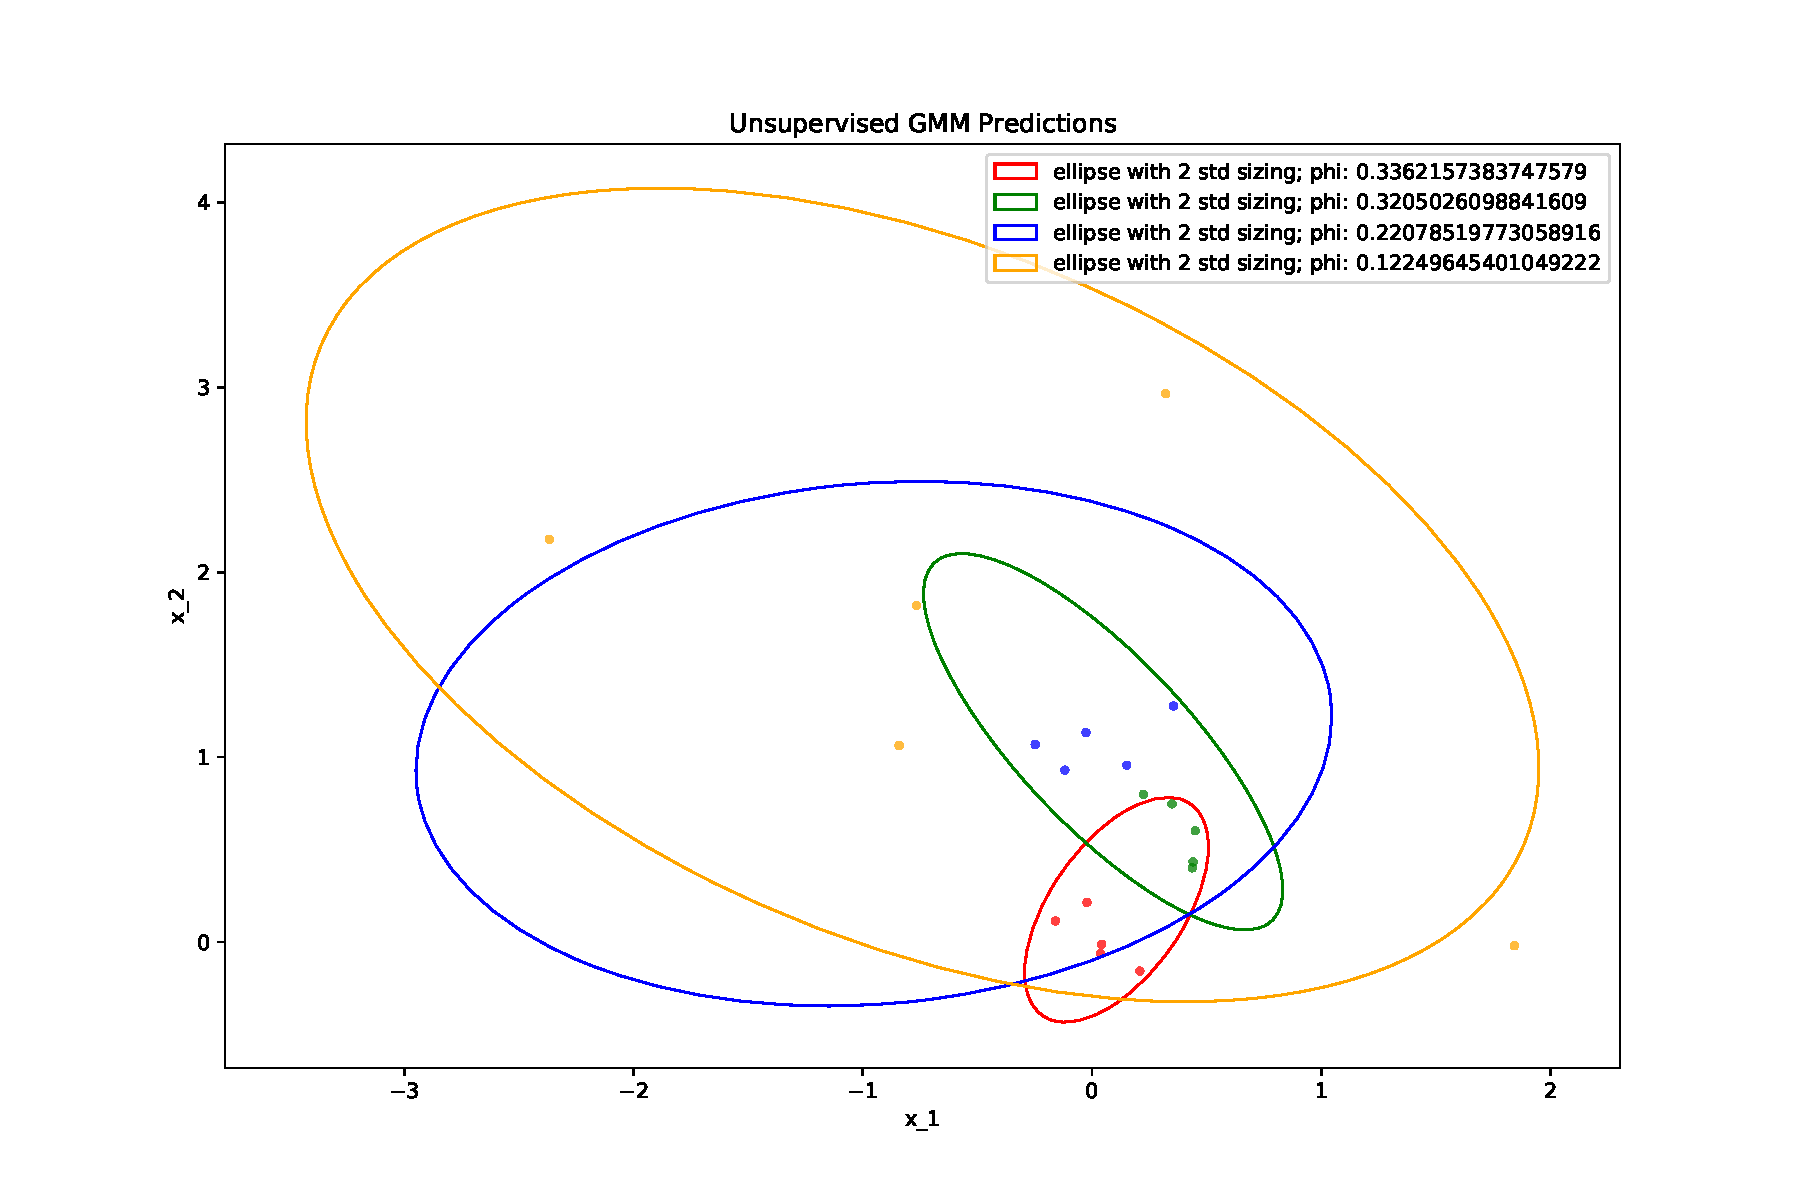
\includegraphics[width=15cm,height=9cm,keepaspectratio]{../src/semi_supervised_em/pred_labelled.pdf}
\end{figure}

Plotting the semi supervised predicted gaussian distributions against the 20 labelled points, and noting the note on the true distribution being 3 low variance gaussians and one high variance. So we see that the semi supervised prediction was better in capturing this than the unsupervised, but still not perfect - it only hits 2 out of the 3 low variance gaussians. We see that it mistakenly has the blue labelled points' ellipse blown up much bigger than the low variance. We somehow ended up with the red ellipse cannabilising some of the unlabelled green points, the green ellipse totally cannabilising the unlabelled blue points, and the blue ellipse left to blow up massively, still covering okishly its' labelled blue points.

The problem above is the small number of supervised points, only 20 compared to 980 unsupervised. At least we have a good spread between clusters.
We can try to fix this by adjusting the weight $\alpha$, increasing it to try to force the blue gaussian smaller to truly capture its cluster. This works - plotted are for $\alpha=40$ and $\alpha=80$ - we see the blue gaussian shrinking and then subsequently pretty well fitting its true cluster

\begin{figure}[H]
	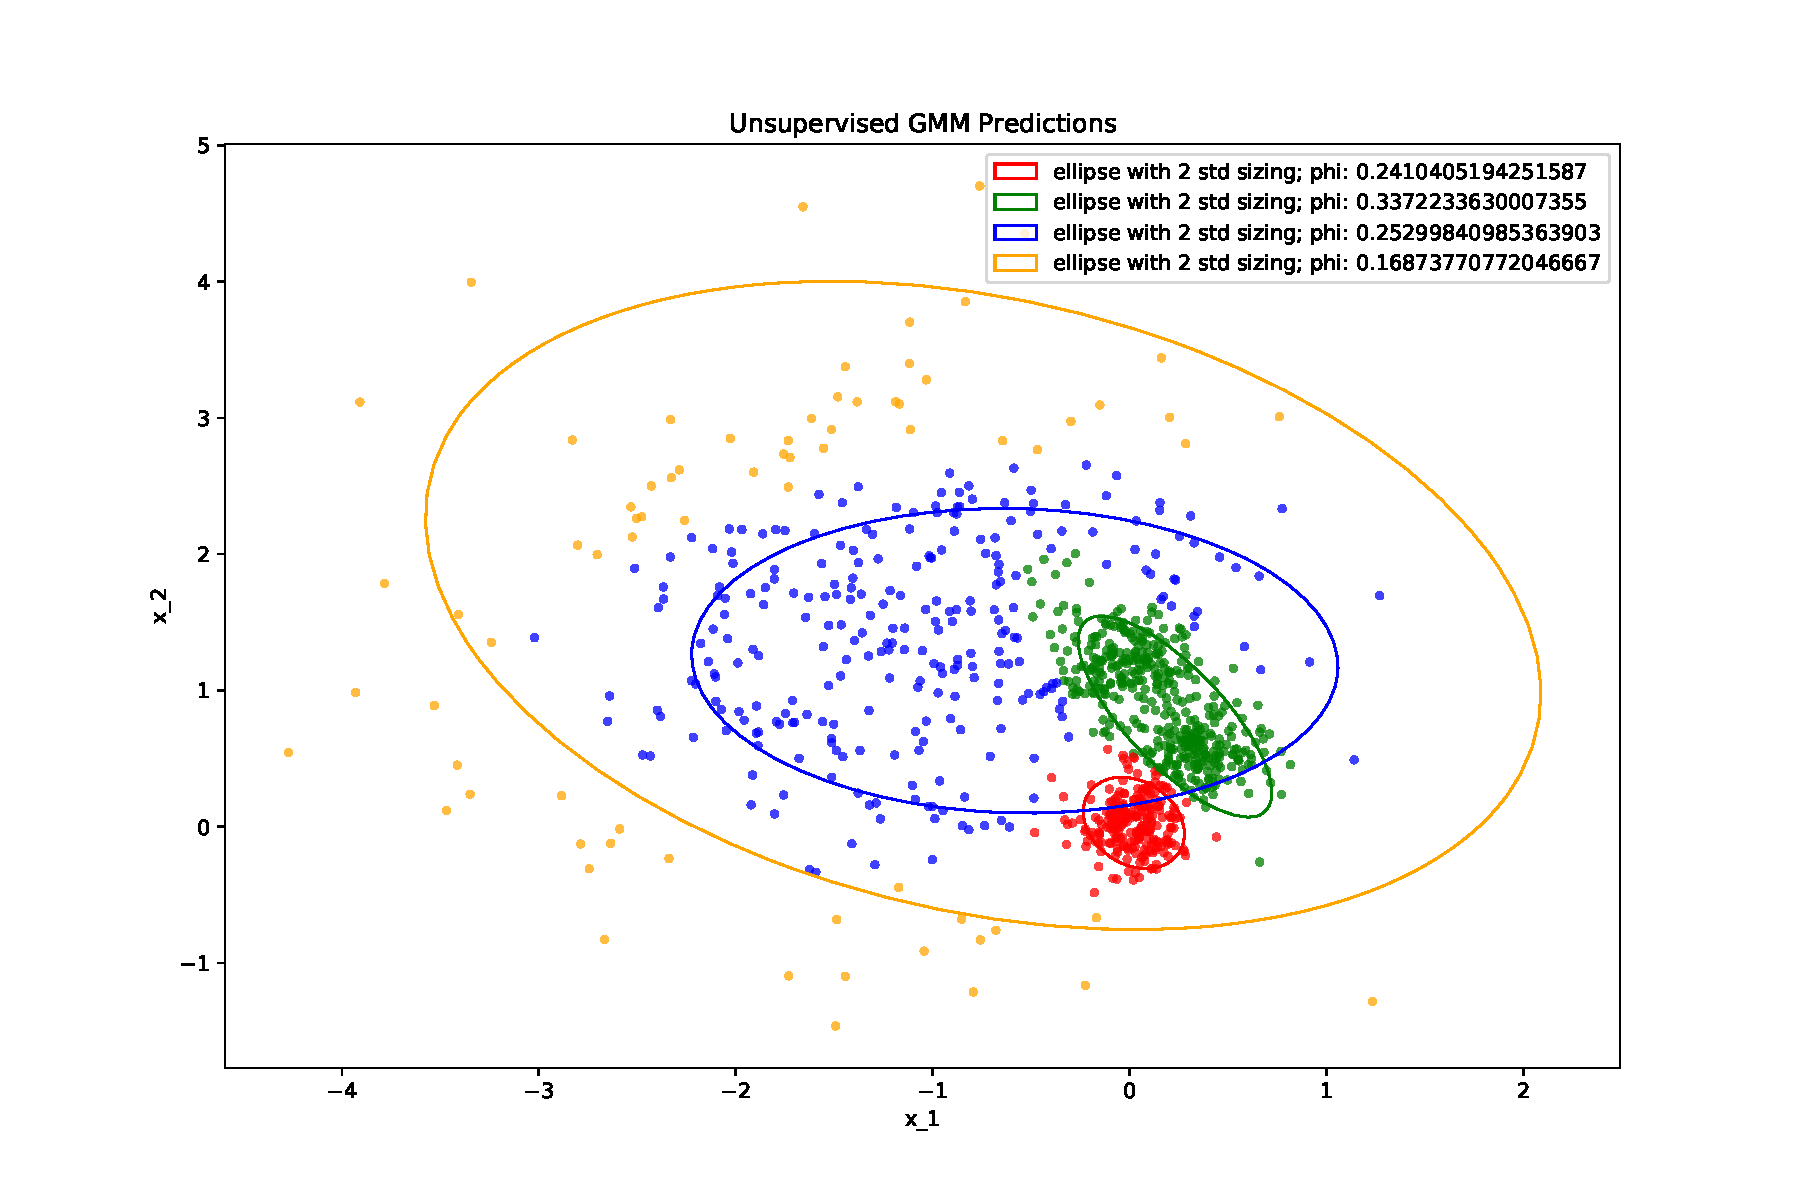
\includegraphics[width=15cm,height=9cm,keepaspectratio]{../src/semi_supervised_em/pred_alpha_40_ss.pdf}
\end{figure}

\begin{figure}[H]
	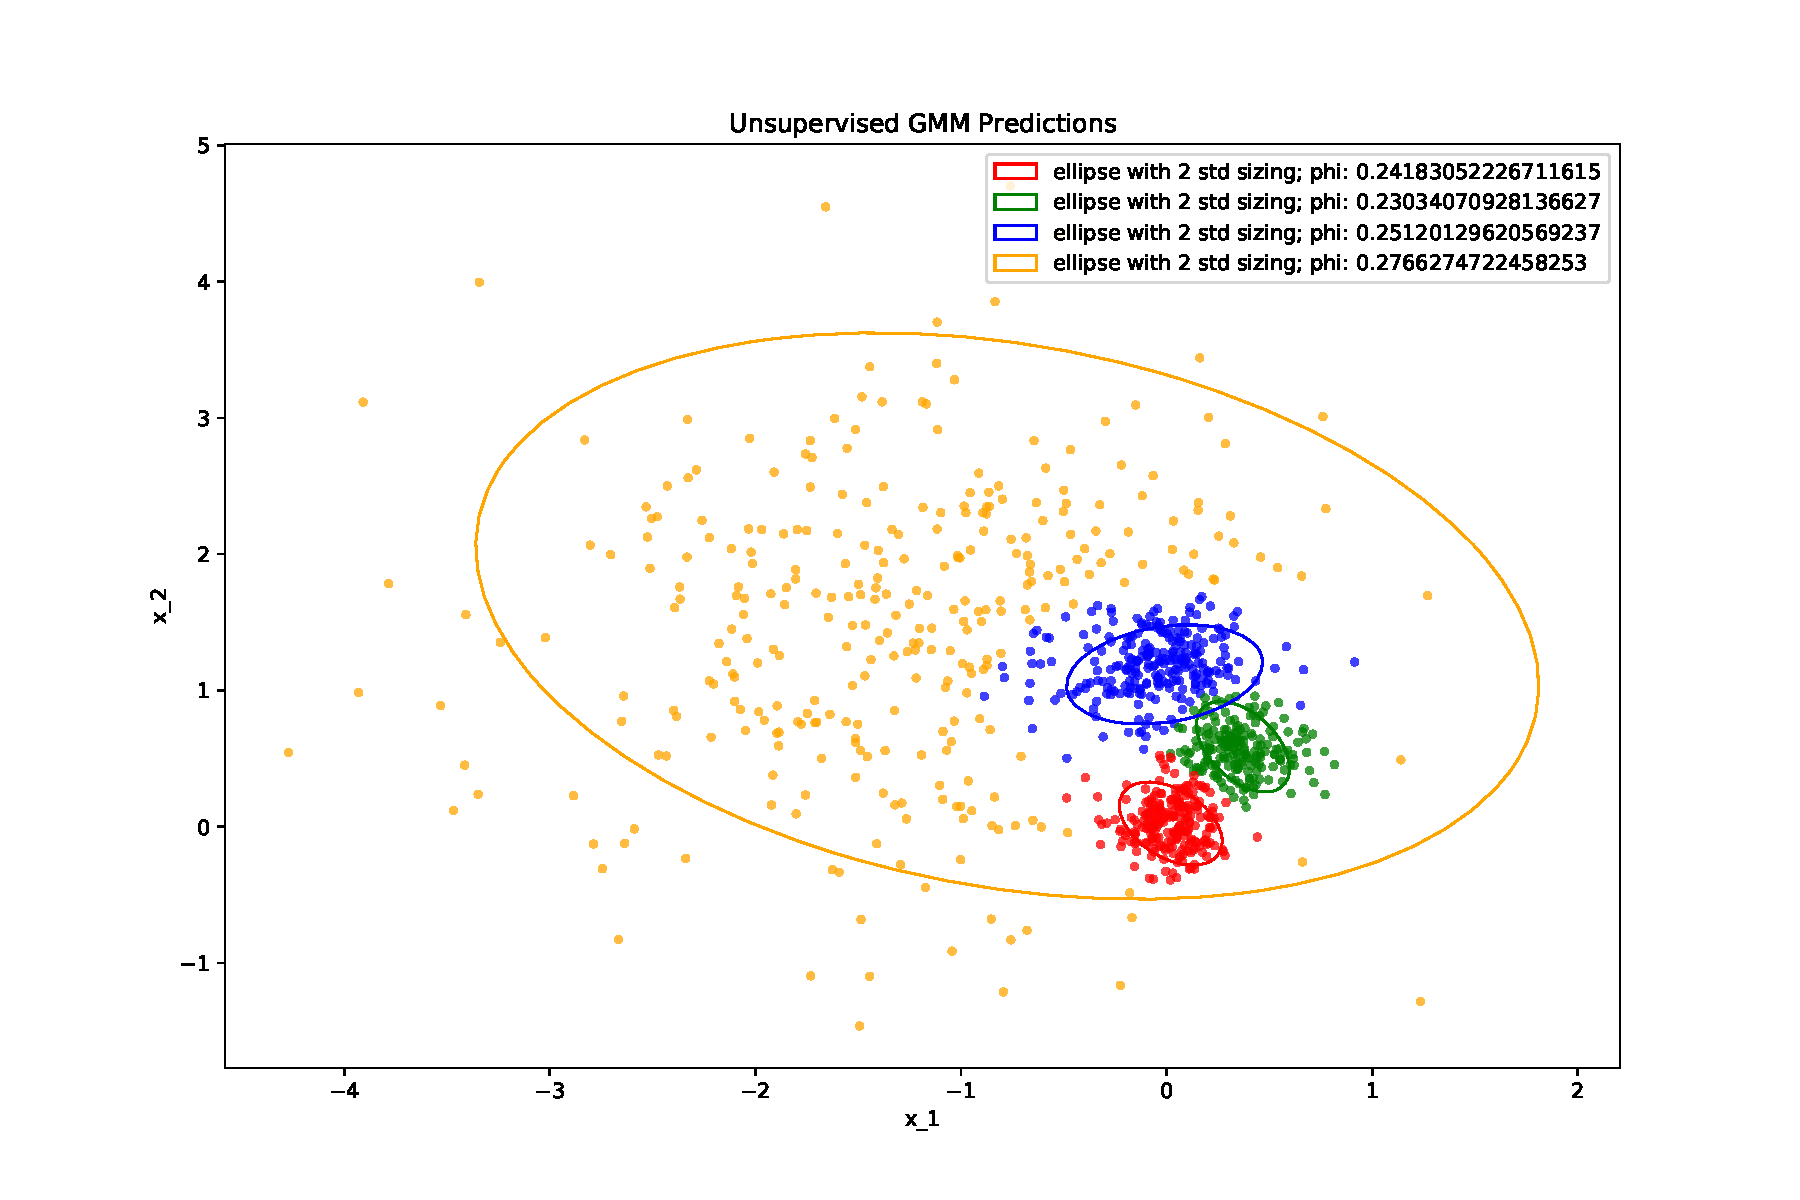
\includegraphics[width=15cm,height=9cm,keepaspectratio]{../src/semi_supervised_em/pred_alpha_80_ss.pdf}
\end{figure}

\end{answer}

} \fi

\end{enumerate}
